\documentclass{kul-ulille-beamer}
%\setbeameroption{show notes on second screen=right} % Both

% TODO
% Move notes to slides
% Introduce decoding from spatiotemporal nature of ERP
% Merge 1. and 2. into 'bci design' to declutter
% Backup slides for all reviewers based on review questions
% Go through old frames
% Go through comments presentation Lille
% Go through comments Hakim
% check dissertation for conclusions, limitations, recap (conclusion per topic)
% and perspectives


%% Preamble ===================================================================
\usepackage{defense}

\addbibresource{references.bib}

\title{%
  A visual Brain-Computer Interface \\
  for gaze-free communication
}
\author{Arne Van Den Kerchove}
\date{December 16, 2024}

\begin{document}

% =============================================================================

\titleframe

% =============================================================================

\begin{frame}
  \frametitle{The Locked-in Syndrome}
  \centering
  {\Large A functioning mind trapped in a paralyzed  body}
  \bigskip
  \bigskip

  \begin{minipage}[b]{.5\textwidth}
    \includegraphics[width=\textwidth]{figures/intro/damien.jpg}
  \end{minipage}\hfill%
  \begin{minipage}[b]{.4\textwidth}
    Severe paralysis leads to \\
    \emph{Locked-in Syndrome}, due to
    \begin{itemize}
      \item Stroke
      \item Traumatic brain injury
      \item Neurodegenerative diseases
      \item \ldots
    \end{itemize}
  Communication requires \\ \emph{assistive technology}
  \end{minipage}
\end{frame}


\note{%
  \begin{itemize}
    \item Some people cannot communicate
    \item Lis:  loss of nearly all voluntary control over muscles.
    \item no speech or typing
    \item require assistive technology
    \item improve QoL
    \item like eye tracker or muscle controlled switch, depending on residual
      control and impairment cannot always use this

    % TODO: Damiens story
  \end{itemize}
}
%
\begin{frame}
  \frametitle{The Brain-Computer Interface}
  \schema{figures/intro/bci.pdf}
\end{frame}


\begin{frame}[c]
  \frametitle{Research question}
  \centering

  \begin{minipage}{.8\textwidth}
  \centering
  \huge
  How can we optimize \emph{BCI}  assistive technology design  to make it more
    \emph{efficient} and  \emph{inclusive}?
  \end{minipage}

\end{frame}

\note{
  inclusive: more people can use it
}

\outline{Outline}{figures/outline.pdf}


% =============================================================================

\outline{1. BCI design}{figures/outline_design.pdf}

\begin{frame}[c]
  \frametitle{Recording the brain activity}
  \schema{figures/intro/recording_modalities.pdf}
  \hfill
  \aside{%
    \emph{EEG}  measures the \\ electrical field on the
    scalp:
    \begin{itemize}
      \item[\textcolor{mygreen}{+}] Non-invasive
      \item[\textcolor{mygreen}{+}] Cheap
      \item[\textcolor{myred}{--}] Limited resolution
      \item[\textcolor{myred}{--}] Low signal-to-noise ratio
    \end{itemize}
  }
\end{frame}
% TODO: de clue: we moeten met deze ruis omgaan in paradigm and decoder design


% TODO: je kan de hersenactiviteit wel opnemen, maar dat is pas nuttig als de
% gebruiker een bepaalde taak aan het uitvoeren is zodat we weten welke
% activiteit we eruit moeten halen

\begin{frame}
  \frametitle{BCI paradigms}
  \begin{minipage}[c]{.5\textwidth}
    \footnotesize
    \sffamily
\begin{tikzpicture}[
    scale=\textwidth/3cm,
  ]
  %\useasboundingbox (-1,-1.25) rectangle (1,1);
  \pgfmathsetmacro{\margin}{.1}
  \pgfmathsetmacro{\center}{.5+.5*\margin}
  \pgfmathsetmacro{\textspacing}{.15}
  %\begin{scope}[shift={(1,1.2)}]
    % Draw axes
    \draw[mydarkgray, very thick, <->] ({-(1+\margin)}, 0) -- ({1+\margin},0);
    %\draw[mydarkgray, very thick, <->] (0,{-(1+\margin)}) -- (0,{1+\margin});

    % Draw rectangles
    \draw[draw=accent1!50, fill=white, very thick] ({-\margin}, \margin) rectangle (-1,1);
    \draw[draw=accent2, fill=white, very thick] (\margin, \margin) rectangle (1,1);
    %\draw[draw=accent3!50, fill=white, very thick] (-1, {-\margin}) rectangle (1,-1);

    %% Add text
    \node[color=accent1!50, align=left,font=\bfseries, anchor=north west, inner sep=2pt] at  (-1,1){Active};
    \node[color=accent2, align=left,font=\bfseries, anchor=north east, inner sep=2pt] at  (1,1){Reactive};
    %\node[color=accent3!50, align=left,font=\bfseries, anchor=south west, inner sep=2pt] at  (-1,-1){Passive};

    %\node[color=mydarkgray, align=center,font=\bfseries, anchor=north] at
    %(0,{-(1+\margin)}) {passive\\participation};
    %\node[color=mydarkgray, align=center,font=\bfseries, anchor=south] at
    %(0,{1+\margin}) {active\\participation};
    \node[color=mydarkgray, align=center,font=\bfseries, anchor=east] at ({-(1+\margin)}, 0) {stimulus\\independent};
    \node[color=mydarkgray, align=center,font=\bfseries, anchor=west] at ({1+\margin},0) {stimulus\\dependent};

    %% Text in rectangles
    \node[align=center] at ({-\center}, {\center-\textspacing}) {movement};
    \node[align=center] at ({-\center}, {\center+\textspacing}) {speech};
    %\node[align=center] at ({-\center}, {\center-1.5*\textspacing}) {neurofeedback};

    \node[align=center] at ({\center}, {\center-1.3*\textspacing}) {tactile};
    \node[align=center] at ({\center}, {\center}) {auditory};
    \node[align=center] at ({\center}, {\center+1.3*\textspacing}) {visual};
    %\node[align=center] at ({\center-\textspacing}, {\center-\textspacing}) {mVEP};

    %% More text
    %\node[align=center] at ({\center}, {-\center+\textspacing}) {error\\potentials};
    %\node[align=center] at ({-\center}, {-\center+\textspacing}) {attention and \\ workload detection};
    %\node[align=center] at ({-\center}, {-\center-\textspacing}) {clinical neuroimaging \\ and monitoring};
    %\node[align=center] at ({+\center}, {-\center-\textspacing})  {emotion \\ detection};
    %\node[align=center] at (0, {-\center})  {$\cdots$};
  %\end{scope}
\end{tikzpicture}

  \end{minipage}\hfill%

  \aside{%
    \small
    \emph[accent3]{Passive} BCIs
      \begin{itemize}
        \footnotesize
        \item[\textcolor{myred}{--}] Less practical
      \end{itemize}
      \smallskip

      \emph[accent1]{Active} BCIs
      \begin{itemize}
        \footnotesize
        \item[\textcolor{mygreen}{+}] Intuitive, self-paced
        \item[\textcolor{myred}{--}] High speed requires invasive
      \end{itemize}
      \smallskip

      \emph[accent2]{Reactive} BCIs decode reactions to attended stimuli%
      \begin{itemize}
        \footnotesize
        \item[\textcolor{myred}{--}] Less intuitive
        \item[\textcolor{mygreen}{+}] Fast stimulation
        \item[\textcolor{mygreen}{+}] Suited for EEG
      \end{itemize}
      \emph{Visual} is fastest
    }
\end{frame}
\note{%
  %TODO: Goal: fast transfering of information in communication assisted technology
  \begin{itemize}
    \item categorized participation and stimulation
    \item performing a specific task
    \item brain activity from task can be decoded
    \item passive less useful
  \end{itemize}
}
%TODO: stimuli represent discrete choices, e.g.virtual keyboard

\begin{frame}
  \frametitle{The visual event-related potential  paradigm}
  % TODO: switch bottom top
  \begin{minipage}[c]{.4\textwidth}
    \begin{tikzpicture}
      \node at (current page.north east) [%
        anchor=north east,
        text width=7cm,
        fill=white, opacity=1,
        xshift=1cm,
        yshift=-.5cm,
        thin
      ]{%
        \input{figures/intro/erp.tikz.tex}
      };
    \end{tikzpicture}
    \smallskip

    \includegraphics[width=\textwidth]{figures/intro/oddball.pdf}
  \end{minipage}\hfill%
  \begin{minipage}[c]{.5\textwidth}
    \begin{enumerate}
      \item Stimuli flash one by one
      \smallskip
      \item Flashes evoke ERPs
      \smallskip
      \item User attends a stimulus
      \smallskip
      \item ERP components are \\ modulated by attention
      \smallskip
      \item Decode target based on \\ timing and components
    \end{enumerate}
  \end{minipage}
\end{frame}


% =============================================================================

\outline{3. Spatiotemporal ERP decoding}{figures/outline_decode.pdf}
\begin{frame}[c]
  \frametitle{\emph{Problem:} ERPs are high dimensional features}
  \begin{minipage}[c]{.5\textwidth}
    Machine learning models must be \\ trained to decode ERPs
    \begin{itemize}
      \item Low single-trial signal-to-noise ratio
      \item High number of features \\ (channels $\times$ times)
      \item Short calibration time \\ results in low sample size
    \end{itemize}
    \bigskip

    \centering
    \emph{\# features $>>$ \# samples}

  \end{minipage}\hfill%
  \begin{minipage}[c]{.4\textwidth}
    \raggedleft

    \includegraphics[width=\textwidth]{figures/bttda/tensor_st.pdf}

  \end{minipage}
\end{frame}

\begin{frame}[c]
  \frametitle{Retaining space-time structure enhances performance}
  \begin{minipage}[c]{.5\textwidth}
    \begin{itemize}
      \item Data are ususally flattened \\ before classification
      \item Spatiotemporal structure is often ignored
    \end{itemize}
    \bigskip

    Assumptions on \emph{data structure}
    \begin{itemize}
      \item yield strong regularization
      \item speed up training
    \end{itemize}
  \end{minipage}\hfill%
  \begin{minipage}[c]{.4\textwidth}
    \raggedleft
    \includegraphics[width=.9\textwidth]{figures/bttda/tensor_flat.pdf}
    \bigskip

    \includegraphics[width=\textwidth]{figures/bttda/tensor_st.pdf}

  \end{minipage}
\end{frame}

\begin{frame}[c]
  \frametitle{Covariance matrix regularization
  {\tiny\cite{VanDenKerchove2022}}}


\end{frame}

\begin{frame}
  \frametitle{Tensor feature extraction {\tiny\cite{VanDenKerchovesubmitted}}}

  \begin{minipage}[t]{.35\linewidth}
    Tensor discriminant analysis
    \bigskip

		\centering
		\begin{tikzpicture}[y=-1cm]
			\begin{scope}[shift={(-1,0)}]
				\TensorThree{$\ten{X}$}{}{}{}{1}{2}{1}
				\node at (2.5,.5, 2) {$\rightarrow$};
				\begin{scope}[shift={(3,0)}]
					\TensorThree{$\ten{G}$}{}{}{}{1}{1}{1}
				\end{scope}
				\node at (4.1,1.1, 2) {$\downarrow$};
				\begin{scope}[shift={(3,2)}]
					\TensorTwo{\textit{clf}}{}{}{1.5}{.5}
				\end{scope}
			\end{scope}
    \end{tikzpicture}
    {\tiny\cite{Phan2010}}
	\end{minipage}\hfill%
  \vrule\hfill%
  \begin{minipage}[t]{.55\textwidth}
    Block-term tensor discriminant analysis
    \bigskip

    \centering
		\begin{tikzpicture}[y=-1cm]
			\begin{scope}[shift={(-1,0)}]
				\TensorThree{$\ten{X}$}{}{}{}{1}{2}{1}
				\node at (2.5,.5, 2) {$\rightarrow$};
				\begin{scope}[shift={(3,0)}]
					\TensorThree{$\ten{G}^{(1)}$}{}{}{}{1}{1}{1}
				\end{scope}
				\node at (5.5,.5,2) {$,\cdots,$};
				\begin{scope}[shift={(6,0)}]
					\TensorThree{$\ten{G}^{(B)}$}{}{}{}{1}{1}{1}
				\end{scope}
				\node at (4.1,1.1, 2) {$\downarrow$};
				\node at (5.6,1.1, 2) {$\downarrow$};
				\node at (7.1,1.1, 2) {$\downarrow$};
				\begin{scope}[shift={(3,2)}]
					\TensorTwo{\textit{clf}}{}{}{4.5}{.5}
				\end{scope}
			\end{scope}
    \end{tikzpicture}

    \begin{itemize}
      \itemposi More flexible
      \itemposi Still retains structure
      \itemnega More hyperparameters
      \item Heuristic model selection
      \item Validated with 4 open datasets
    \end{itemize}
  \end{minipage}

\end{frame}
\note{
  Another method: consider that we keep all data in its original shape and find
  separate transformations for space and for time
}


% =============================================================================

\outline{4. Gaze-independence}{figures/outline_gaze.pdf}


\begin{frame}
  \frametitle{\emph{Problem:} Eye motor impairment \\  prevents gazing at targets}

  \begin{minipage}[c]{.4\textwidth}
    \raggedright
    \emph{Visual skills} related to disease \\ affect BCI
    operation
    {\tiny\cite{FriedOken2020}}
  {\small
  \begin{itemize}
    \item Discomfort fixating
    \item Restricted movement
    \item Involuntary movements
  \end{itemize}
  }
  \bigskip

  Decoding relies on \emph{visual ERP} components {\tiny\cite{Treder2010}}
	\end{minipage}\hfill%
  \begin{minipage}[c]{.4\textwidth}
    \vspace{-1cm}
		\centering
		\includegraphics[width=.7\textwidth]{figures/intro/covert_performance_drop/brunner_2010_line.png}

    \raggedleft
    {\tiny\cite{RonAngevin2019}}
    \bigskip


    \framebox{\parbox{\textwidth}{%
    \centering
    Those who can't use eye \\ tracking need BCIs
    \smallskip

    \emph{but}
    \smallskip

    Visual BCIs perform poorly
    }}


	\end{minipage}
\end{frame}

\note{
  \begin{itemize}
    \item Explain axes
    \item Accuracy is lower when not gazing directly
    \item Even below 80\% usability threshold
  \end{itemize}

}


\begin{frame}
  \frametitle{Covert visuospatial attention experiment}

  \begin{minipage}{.6\textwidth}
    \centering

    \begin{minipage}[t]{.45\textwidth}
    \input{figures/covert/interface_3.tikz.tex}
    \end{minipage}\hfill%
    \begin{minipage}[t]{.45\textwidth}
      \includegraphics[width=\textwidth]{example-image}

      timeline
    \end{minipage}
    \bigskip
    \bigskip
    \bigskip


    {\small
    \begin{minipage}{.3\textwidth}
      \emph{Overt} VSA
      \smallskip

      \includegraphics[width=\textwidth]{figures/covert/attention_overt.pdf}
    \end{minipage}\hfill%
    \begin{minipage}{.3\textwidth}
      \emph{Covert} VSA
      \smallskip

      \includegraphics[width=\textwidth]{figures/covert/attention_covert.pdf}
    \end{minipage}\hfill%
    \begin{minipage}{.3\textwidth}
      \small
      \emph{Split} VSA
      \smallskip

      \includegraphics[width=\textwidth]{figures/covert/attention_split.pdf}
    \end{minipage}%
  }
  \end{minipage}\hfill

  \aside{%
    \small
    \raggedright
    CVSA-ERP dataset
    \begin{itemize}
      \item 15 subjects, $\pm$ 11h stimulation
      \item Hex-o-Spell interface \\ {\tiny\cite{Treder2010}}
      \item Discrete gaze-\\independence conditions
    \end{itemize}
    \raggedright
    {\tiny\cite{VanDenKerchove2024}}
  }
\end{frame}
\note{
  Hex-o-Spell optimized for gaze-independence
}

\begin{frame}
  \frametitle{Evoked ERP components}
  \small
  \begin{minipage}[t]{.45\textwidth}
    \includegraphics[width=.2\textwidth]{figures/covert/attention_overt.pdf}
    \hspace{.5em}
    \emph{Overt} VSA
    \smallskip

    \includegraphics[width=\textwidth]{figures/covert/erps/erp_overt_cluster-1.pdf}
    \includegraphics[width=\textwidth]{figures/covert/erps/erp_overt_cluster-0.pdf}
    \smallskip

    \small
    F-statistic cluster-based permutation \\ tests, target vs. non-target
  \end{minipage}\hfill%
  \begin{minipage}[t]{.45\textwidth}
    \includegraphics[width=.2\textwidth]{figures/covert/attention_covert.pdf}
    \hspace{.5em}
    \emph{Covert} VSA
    \smallskip

    \includegraphics[width=\textwidth]{figures/covert/erps/erp_covert_cluster-0.pdf}
    \smallskip

    \includegraphics[width=.2\textwidth]{figures/covert/attention_split.pdf}
    \hspace{.5em}
    \emph{Split} VSA
    \smallskip

    \includegraphics[width=\textwidth]{figures/covert/erps/erp_split_cluster-0.pdf}

  \end{minipage}
\end{frame}


%% =============================================================================

\outline{5. Gaze-independent decoding}{figures/outline_decode.pdf}

\begin{frame}[c]
  \frametitle{\emph{Problem:} Latency jitter decreases performance \\ in covert and split
  attention}
  \begin{minipage}{.4\textwidth}
    \centering
\small

\begin{tikzpicture}   % First subplot (low jitter) positioned relative to center
    \begin{axis}[
        at={(0,0)}, % Adjust position to the left, closer to the center
        anchor=center,
        width=\textwidth, height=.7\textwidth,
        xmin=20, xmax=80,
        ymin=-0.1, ymax=1.1,
        axis lines=none, % Remove axes
        title={low jitter}, % Add title
        title style={yshift=-10pt, color=muteblack}, % Adjust title position to make it closer to the plot
        ]
        % Plot individual waveforms (low jitter) in darkgray
        \addplot[darkgray,domain=20:80,samples=100] {exp(-0.5*((x-50)/5)^2)};
        \addplot[darkgray,domain=20:80,samples=100] {exp(-0.5*((x-52)/5)^2)};
        \addplot[darkgray,domain=20:80,samples=100] {exp(-0.5*((x-48)/5)^2)};
        \addplot[darkgray,domain=20:80,samples=100] {exp(-0.5*((x-51)/5)^2)};
        \addplot[darkgray,domain=20:80,samples=100] {exp(-0.5*((x-49)/5)^2)};

        % Plot average waveform (low jitter) in accent1 color, very thick
        \addplot[ultra thick,accent1,domain=20:80,samples=100] {exp(-0.5*((x-50)/5)^2)};
    \end{axis}
\end{tikzpicture}
\bigskip

\begin{tikzpicture}

   % Second subplot (high jitter) positioned relative to center
   \begin{axis}[
      at={(0.55\textwidth,0)}, % Adjust position to the left, closer to the center
       anchor=center,
        width=\textwidth, height=.7\textwidth,
       xmin=20, xmax=80,
       ymin=-0.1, ymax=1.1,
       axis lines=none, % Remove axes
       title={high jitter}, % Add title
       title style={yshift=-10pt, color=muteblack}, % Adjust title position to make it closer to the plot
       ]
       % Plot individual waveforms (high jitter) in darkgray
       \addplot[darkgray,domain=20:80,samples=100] {exp(-0.5*((x-45)/5)^2)};
       \addplot[darkgray,domain=20:80,samples=100] {exp(-0.5*((x-55)/5)^2)};
       \addplot[darkgray,domain=20:80,samples=100] {exp(-0.5*((x-40)/5)^2)};
       \addplot[darkgray,domain=20:80,samples=100] {exp(-0.5*((x-60)/5)^2)};
       \addplot[darkgray,domain=20:80,samples=100] {exp(-0.5*((x-50)/5)^2)};

       % Plot average waveform (high jitter) in accent1 color, very thick
       \addplot[ultra thick,accent1,domain=20:80,samples=100] {0.2*(exp(-0.5*((x-45)/5)^2) + exp(-0.5*((x-55)/5)^2) + exp(-0.5*((x-40)/5)^2) + exp(-0.5*((x-60)/5)^2) + exp(-0.5*((x-50)/5)^2))};
   \end{axis}
\end{tikzpicture}%
\bigskip

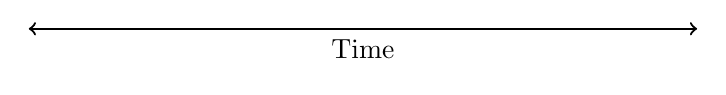
\begin{tikzpicture}
    % Draw the bottom horizontal axis
    \draw[thick,<->] (-0.35\textwidth,-1) -- (.35\textwidth,-1) node[pos=0.5,below] {Time};
\end{tikzpicture}
%\vspace{-5cm}

  \end{minipage}\hfill%
  \begin{minipage}{.55\textwidth}
    \small
    \centering
    {\centering\resizebox{.7\textwidth}{!}{%
    \small
    %CVSA-ERP (our dataset) \hspace{3.5em} BNCI2014-009
    %\smallskip

    \input{figures/covert/jitter.pgf}
    }}
    \smallskip

    \begin{itemize}
      \item Classifier-based latency estimation {\tiny\cite{Mowla2017}}
      \item Jitter of discriminative information is higher
        for gaze-independent settings
      \item Contributes to low accuracy {\tiny\cite{Arico2014}}
      \item \emph{Can this be exploited?}
    \end{itemize}

  \end{minipage}

\end{frame}
\note{
  Using a technique called CBLE extract latencies of single-trial ERPs
}

\begin{frame}
  \frametitle{Latency estimation and alignment}
\end{frame}

\begin{frame}
  \frametitle{Alignment of simulated data}
  \begin{minipage}{.45\textwidth}
    \raggedright
    \emph{Before} alignment
    \smallskip

    \includegraphics[width=\textwidth, height=\textwidth]{example-image-a}
  \end{minipage}\hfill%
  \begin{minipage}{.45\textwidth}
    \raggedright
    \emph{After} alignment
    \smallskip


    \includegraphics[width=\textwidth, height=\textwidth]{example-image-b}
  \end{minipage}
\end{frame}
\note{
  To test, we must know the true latencies, so simulated data
}

\begin{frame}
  \frametitle{Application to gaze-independent decoding}
  \begin{minipage}{.6\textwidth}
    \centering
    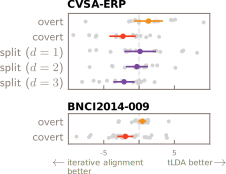
\includegraphics[width=\textwidth]{figures/covert/roc_auc_diff.pdf}
  \end{minipage}\hfill
  \aside{%
    WCBLE can function with unseen data and is applicable as decoder
    \bigskip

    Within-subject, cross-validated single-trial ROC-AUC (\%)
    \bigskip

    Within and across VSA conditions to establish independence
    \bigskip

    Improves decoding performance in gaze-independent settings


  }
\end{frame}
\note{Across: transfer}

% =============================================================================

\outline{6.Evaluation in end-users}{figures/outline_patient.pdf}
\note{
  Now proposed a way to enhance gaze-independent decoding as a proposed
  solution for individuals with eye motor impairment
}

\begin{frame}
  \frametitle{Subjects with physical, speech and gaze impairment}
  \centering
  \includegraphics[width=.6\textwidth]{example-image}
\end{frame}

\begin{frame}
  \frametitle{Eye motor impairment}
  \centering
  \includegraphics[width=.6\textwidth]{example-image}
\end{frame}

\begin{frame}
  \frametitle{Off-line covert vsa experiment}
  photo of setup

  pictures of conditions

\end{frame}

\begin{frame}
  \frametitle{Gaze tracking analysis}
  Most prefered to perform overt VSA, despite severe eye motor impairment

  Eye tracking  with portable eye tracker could not properly be established due
  to eye motor impairments
\end{frame}

\begin{frame}
  \frametitle{Subject decoding performance}
  Who/how many performed above chance?
  Did WCBLE matter? -> not that much, only when TODO
\end{frame}



%% =============================================================================
%
%\begin{frame}[c]
%    \centering
%    \Large
%
%    Balance the bandwidth of a \emph{visual ERP BCI} with the \\needs
%    of individuals with \emph{eye motor impairment} \\ through \emph{improving
%    decoding} of covert attention.
%\end{frame}
%\note{
%
%  Almost a contradiction: patients are completely paralysed with no motor
%  output, even from the eyes to the point where they cannot use an eye tracker.
%  So we propose a BCI for them as a supposedly independent communication means
%  that does not require any muscle control. Yet, exactly in these cases spatial visual
%  ERP bcis perform poorly.
%}
%
%\tocframeall
%\section{\textbf{C1}: General ERP decoding algorithms}
%\tocframe
%
%\begin{frame}[c]
%  \frametitle{Exploit channel-time structure of ERP data \\ for regularization}
%  \begin{minipage}[c]{.4\textwidth}
%    \centering
%    \includegraphics[width=\textwidth]{figures/bttda/tensor_st.pdf}
%  \end{minipage}\hfill%
%  \begin{minipage}[c]{.4\textwidth}
%    \centering
%    \includegraphics[width=\textwidth]{figures/bttda/tensor_flat.pdf}
%  \end{minipage}
%\end{frame}
%
%
%\begin{frame}[c]
%	\frametitle{Higher-order discriminant analysis}
%	\centering
%	\begin{tikzpicture}[y=-1cm]
%		\TensorThree{$\ten{X}$}{}{}{}{2}{2}{1}
%		\begin{scope}[shift={(-1.1,0)}]
%			\TensorTwo{$\mat{W}_1$}{}{}{1}{2}
%		\end{scope}
%		\begin{scope}[shift={(0,2.1)}]
%			\TensorTwo{$\mat{W}_2$}{}{}{2}{1}
%		\end{scope}
%		\node at (3.3,.5, 2) {$=$};
%		\begin{scope}[shift={(4,0)}]
%			\TensorThree{$\ten{G}$}{}{}{$N$}{1}{1}{1}
%		\end{scope}
%	\end{tikzpicture}
%
%	\bigskip
%
%  $\ten{G} = \ten{X}\times_1\mat{W}_1\cdots\times_{K-1}\mat{W}_{K-1}$ \\
%  s.t. $\ten{G}$ is maximally \emph{discriminant}
%	between classes.
%\end{frame}
%
%\begin{frame}[c]
%	\frametitle{HODA and the Tucker tensor core model}
%
%	\begin{minipage}{.4\linewidth}
%		\centering
%    \emph{Tucker} model
%
%		\bigskip
%
%
%		\begin{tikzpicture}[y=-1cm]
%			\begin{scope}[shift={(-1,0)}]
%				\TensorThree{$\ten{X}$}{}{}{}{1}{2}{1}
%				\node at (2.5,.5, 2) {$\rightarrow$};
%				\begin{scope}[shift={(3,0)}]
%					\TensorThree{$\ten{G}$}{}{}{}{1}{1}{1}
%				\end{scope}
%				\node at (4.1,1.1, 2) {$\downarrow$};
%				\begin{scope}[shift={(3,2)}]
%					\TensorTwo{\textit{clf}}{}{}{1.5}{.5}
%				\end{scope}
%			\end{scope}
%		\end{tikzpicture}
%	\end{minipage}\hfill%
%	\begin{minipage}{.5\linewidth}
%		Strong assumptions\\
%		on data structure
%		\begin{itemize}
%			\item[\textcolor{mygreen}{+}] Efficient
%			\item[\textcolor{mygreen}{+}] Regularizing constraints
%			\item[\textcolor{mygreen}{+}] Increased flexibility
%				\smallskip
%
%      \item[\textcolor{myred}{--}] \sout{Redundant features}
%      \item[\textcolor{myred}{--}] \sout{More parameters to tune}
%		\end{itemize}
%	\end{minipage}
%\end{frame}
%
%\begin{frame}[c]
%	\frametitle{Towards a Block-Term Tensor model}
%	\begin{minipage}{.4\linewidth}
%		\centering
%		\textbf{Tucker} model
%
%		\bigskip
%
%		\begin{tikzpicture}[y=-1cm]
%			\begin{scope}[shift={(-1,0)}]
%				\TensorThree{$\ten{X}$}{}{}{}{1}{2}{1}
%				\node at (2.5,.5, 2) {$\rightarrow$};
%				\begin{scope}[shift={(3,0)}]
%					\TensorThree{$\ten{G}$}{}{}{}{1}{1}{1}
%				\end{scope}
%				\node at (4.1,1.1, 2) {$\downarrow$};
%				\begin{scope}[shift={(3,2)}]
%					\TensorTwo{\textit{clf}}{}{}{1.5}{.5}
%				\end{scope}
%			\end{scope}
%		\end{tikzpicture}
%	\end{minipage}\vline%
%	\begin{minipage}{.6\linewidth}
%		\centering
%		\emph{Block-Term Tensor} model
%
%		\bigskip
%
%
%		\begin{tikzpicture}[y=-1cm]
%			\begin{scope}[shift={(-1,0)}]
%				\TensorThree{$\ten{X}$}{}{}{}{1}{2}{1}
%				\node at (2.5,.5, 2) {$\rightarrow$};
%				\begin{scope}[shift={(3,0)}]
%					\TensorThree{$\ten{G}^{(1)}$}{}{}{}{1}{1}{1}
%				\end{scope}
%				\node at (5.5,.5,2) {$,\cdots,$};
%				\begin{scope}[shift={(6,0)}]
%					\TensorThree{$\ten{G}^{(B)}$}{}{}{}{1}{1}{1}
%				\end{scope}
%				\node at (4.1,1.1, 2) {$\downarrow$};
%				\node at (5.6,1.1, 2) {$\downarrow$};
%				\node at (7.1,1.1, 2) {$\downarrow$};
%				\begin{scope}[shift={(3,2)}]
%					\TensorTwo{\textit{clf}}{}{}{4.5}{.5}
%				\end{scope}
%			\end{scope}
%		\end{tikzpicture}
%
%	\end{minipage}
%\end{frame}
%
%\begin{frame}[c]
%	\frametitle{Block-term Tensor Discriminant Analysis}
%
%	\begin{minipage}{.6\linewidth}
%    \centering
%    \emph{Block-term Tensor} model
%
%		\bigskip
%
%    \raggedright
%		\begin{tikzpicture}[y=-1cm]
%			\begin{scope}[shift={(-1,0)}]
%				\TensorThree{$\ten{X}$}{}{}{}{1}{2}{1}
%				\node at (2.5,.5, 2) {$\rightarrow$};
%				\begin{scope}[shift={(3,0)}]
%					\TensorThree{$\ten{G}^{(1)}$}{}{}{}{1}{1}{1}
%				\end{scope}
%				\node at (5.5,.5,2) {$,\cdots,$};
%				\begin{scope}[shift={(6,0)}]
%					\TensorThree{$\ten{G}^{(B)}$}{}{}{}{1}{1}{1}
%				\end{scope}
%				\node at (4.1,1.1, 2) {$\downarrow$};
%				\node at (5.6,1.1, 2) {$\downarrow$};
%				\node at (7.1,1.1, 2) {$\downarrow$};
%				\begin{scope}[shift={(3,2)}]
%					\TensorTwo{\textit{clf}}{}{}{4.5}{.5}
%				\end{scope}
%			\end{scope}
%		\end{tikzpicture}
%	\end{minipage}\hfill%
%	\begin{minipage}{.4\linewidth}
%		Weaker assumptions\\
%		on data structure
%		\begin{itemize}
%
%			\item[\textcolor{mygreen}{+}] Efficient
%			\item[\textcolor{mygreen}{+}] Regularizing constraints
%				\smallskip
%
%      \item[\textcolor{myred}{--}] \sout{Manual rank selection}
%      \item[\textcolor{myred}{--}] \sout{Redundant features}
%      \item[\textcolor{myred}{--}] \sout{Cannot model full covariance structure}
%		\end{itemize}
%	\end{minipage}
%\end{frame}
%
%\begin{frame}[c]
%	\frametitle{Block-term tensor model through deflation}
%	\centering
%	\begin{tikzpicture}[y=-1cm]
%		\TensorThree{$\ten{X}$}{}{}{}{2}{2}{1}
%		\node at (3.3,.5, 2) {$\cong$};
%		\begin{scope}[shift={(6,0)}]
%			\TensorThree{$\ten{G}^{(1)}$}{}{}{}{1}{1}{1}
%		\end{scope}
%		\begin{scope}[shift={(3.9,0)}]
%			\TensorTwo{$\mat{A}_1^{(1)}$}{}{}{2}{1}
%		\end{scope}
%		\begin{scope}[shift={(6,1.1)}]
%			\TensorTwo{$\mat{A}_2^{(1)}$}{}{}{1}{2}
%		\end{scope}
%		\node at (8.6,.5, 2) {$+\cdots+$};
%		\begin{scope}[shift={(12,0)}]
%			\TensorThree{$\ten{G}^{(B)}$}{}{}{}{1}{1}{1}
%		\end{scope}
%		\begin{scope}[shift={(9.9,0)}]
%			\TensorTwo{$\mat{A}_1^{(B)}$}{}{}{2}{1}
%		\end{scope}
%		\begin{scope}[shift={(12,1.1)}]
%			\TensorTwo{$\mat{A}_2^{(B)}$}{}{}{1}{2}
%		\end{scope}
%	\end{tikzpicture}
%
%
%  \emph{Deflation} scheme:
%	%$$\ten{X}^{(0)} = \ten{X}$$
%	$$\ten{X}^{(b+1)} = \ten{X}^{(b)} -
%		\ten{G}^{(b)}\times_1\mat{A}_1^{(b)}\cdots\times_K\mat{A}_K^{(b)}$$
%\end{frame}
%
%\begin{frame}[c]
%  \frametitle{BTTDA oupterforms HODA \\ on benchmark datasets}
%  \includegraphics[width=.7\textwidth]{figures/bttda/blocks.png}%
%  \includegraphics[width=.3\textwidth]{figures/bttda/results_table.png}
%
%\end{frame}
%
%\section{\textbf{C2}: Gaze-independent ERP decoding}
%\tocframe
%\begin{frame}
%  \frametitle{Covert attention ERP \\ data collection}
%  \begin{minipage}{.45\textwidth}
%    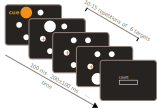
\includegraphics[width=\textwidth]{figures/covert/timeline.pdf}
%  \end{minipage}\hfill%
%  \begin{minipage}{.45\textwidth}
%     CVSA-ERP dataset
%     \begin{itemize}
%       \item $N=15$
%       \item ISI=$300\pm100$ ms
%       \item $\pm$11,25h recoded stimulation,
%       \item 3 conditions based on gaze and attention cue
%     \end{itemize}
%
%    \centering
%    \includegraphics[width=.45\textwidth]{figures/covert/attention_overt.pdf}\hfill%
%    \includegraphics[width=.45\textwidth]{figures/covert/attention_covert.pdf}%
%    \bigskip
%
%    \includegraphics[width=.45\textwidth]{figures/covert/attention_split.pdf}
%  \end{minipage}
%\end{frame}
%
%\begin{frame}
%  \frametitle{Grand average ERPs}
%  TODO: grand average ERPs and F-scores
%\end{frame}
%
%\begin{frame}[c]
%  \frametitle{Latency jitter decreases performance \\ in covert and split
%  attention \tiny\cite{Arico2014}}
%  \begin{minipage}{.4\textwidth}
%    \centering
\small

\begin{tikzpicture}   % First subplot (low jitter) positioned relative to center
    \begin{axis}[
        at={(0,0)}, % Adjust position to the left, closer to the center
        anchor=center,
        width=\textwidth, height=.7\textwidth,
        xmin=20, xmax=80,
        ymin=-0.1, ymax=1.1,
        axis lines=none, % Remove axes
        title={low jitter}, % Add title
        title style={yshift=-10pt, color=muteblack}, % Adjust title position to make it closer to the plot
        ]
        % Plot individual waveforms (low jitter) in darkgray
        \addplot[darkgray,domain=20:80,samples=100] {exp(-0.5*((x-50)/5)^2)};
        \addplot[darkgray,domain=20:80,samples=100] {exp(-0.5*((x-52)/5)^2)};
        \addplot[darkgray,domain=20:80,samples=100] {exp(-0.5*((x-48)/5)^2)};
        \addplot[darkgray,domain=20:80,samples=100] {exp(-0.5*((x-51)/5)^2)};
        \addplot[darkgray,domain=20:80,samples=100] {exp(-0.5*((x-49)/5)^2)};

        % Plot average waveform (low jitter) in accent1 color, very thick
        \addplot[ultra thick,accent1,domain=20:80,samples=100] {exp(-0.5*((x-50)/5)^2)};
    \end{axis}
\end{tikzpicture}
\bigskip

\begin{tikzpicture}

   % Second subplot (high jitter) positioned relative to center
   \begin{axis}[
      at={(0.55\textwidth,0)}, % Adjust position to the left, closer to the center
       anchor=center,
        width=\textwidth, height=.7\textwidth,
       xmin=20, xmax=80,
       ymin=-0.1, ymax=1.1,
       axis lines=none, % Remove axes
       title={high jitter}, % Add title
       title style={yshift=-10pt, color=muteblack}, % Adjust title position to make it closer to the plot
       ]
       % Plot individual waveforms (high jitter) in darkgray
       \addplot[darkgray,domain=20:80,samples=100] {exp(-0.5*((x-45)/5)^2)};
       \addplot[darkgray,domain=20:80,samples=100] {exp(-0.5*((x-55)/5)^2)};
       \addplot[darkgray,domain=20:80,samples=100] {exp(-0.5*((x-40)/5)^2)};
       \addplot[darkgray,domain=20:80,samples=100] {exp(-0.5*((x-60)/5)^2)};
       \addplot[darkgray,domain=20:80,samples=100] {exp(-0.5*((x-50)/5)^2)};

       % Plot average waveform (high jitter) in accent1 color, very thick
       \addplot[ultra thick,accent1,domain=20:80,samples=100] {0.2*(exp(-0.5*((x-45)/5)^2) + exp(-0.5*((x-55)/5)^2) + exp(-0.5*((x-40)/5)^2) + exp(-0.5*((x-60)/5)^2) + exp(-0.5*((x-50)/5)^2))};
   \end{axis}
\end{tikzpicture}%
\bigskip

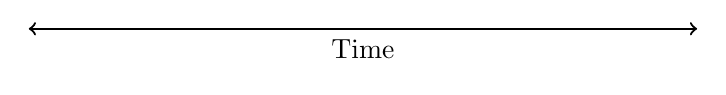
\begin{tikzpicture}
    % Draw the bottom horizontal axis
    \draw[thick,<->] (-0.35\textwidth,-1) -- (.35\textwidth,-1) node[pos=0.5,below] {Time};
\end{tikzpicture}
%\vspace{-5cm}

%  \end{minipage}\hfill%
%  \begin{minipage}{.55\textwidth}
%    \input{figures/covert/jitter.pgf}
%  \end{minipage}
%\end{frame}
%\begin{frame}[c]
%  \frametitle{Classifier-based Latency Estimation with Woody iterations}
%
%  \includegraphics[width=.6\textwidth]{figures/covert/figure1.pdf}
%\end{frame}
%\begin{frame}
%  \frametitle{Aligned vs. non-aligned simulated data}
%\end{frame}
%\begin{frame}
%  \frametitle{Increase in gaze-independent decoding accuracy}
%\end{frame}
%
%\tocframe
%\section{\textbf{C3}: End-user case studies}
%\begin{frame}
%  \frametitle{Experimental setup}
%  \begin{itemize}
%    \item show setup
%    \item list participants
%  \end{itemize}
%\end{frame}
%\begin{frame}
%  \frametitle{Impaired visual skills}
%  show table
%\end{frame}
%\begin{frame}
%  \frametitle{Gaze tracking analysis}
%  highlight specific gaze case
%\end{frame}
%\begin{frame}
%  \frametitle{Usability}
%  how many achieved higher than chance?
%\end{frame}
%\section{Conclusion \& perspectives}


\begin{frame}
  \frametitle{Recap}
  \begin{changemargin}
    \begin{enumerate}
      \item Visual, spatial ERP paradigm
      \item 2 decoders exploiting spatiotemporal structure
      \item Alignment decoder for gaze independence
      \item Covert attention study with healthy subjects
      \item Off-line study with eye-motor impaired patients
    \end{enumerate}
    TODO: main takeaway of each
  \end{changemargin}
\end{frame}

\begin{frame}
    \frametitle{Conclusions}
    \begin{changemargin}
    \begin{itemize}
      \item Improved decoders enhance BCI \emph{efficiency}.
      \item Applications to gaze-independent decoding improve \emph{inclusivity}.
      \item Limited effect on end-users
      \item Gained insight in requirements of BCI users with gaze-impairment
    \end{itemize}
  \end{changemargin}
\end{frame}

\begin{frame}
  \frametitle{Perspectives}
  \begin{changemargin}
    \begin{itemize}

     \item On-line experiments
     \item User experience study
     \item Models capturing multi-component and
       non-stationary aspect of (covert) ERPs
  \end{itemize}
  \end{changemargin}
\end{frame}
\note{
  Once the on-line system is available, this allows us to do a proper user
  experience study
}

\begin{frame}
  \frametitle{Q\&A}
  \centering
	\inserttitlegraphic
\end{frame}
%
%%% BACKUP Slides ==============================================================



% TODO: mathematics
\begin{frame}
  \frametitle{Experimental procedure \\ CVSA-ERP}
  hardware, locations, timings, nr of blocks, ...
\end{frame}
\begin{frame}
  \frametitle{Experimental procedure \\ end-user study}
  hardware, locations, timings, nr of blocks, ...
\end{frame}

\begin{frame}
  \frametitle{Block-term tensor discriminant analysis procedure}
  backward model image and equation

  forward model image and equation

  deflation image and equations

  model selection procedure
\end{frame}

\begin{frame}
  \frametitle{Block-term tensor discriminant analysis procedure}
  backward model image and equation

  forward model image and equation

  deflation image and equations

  model selection procedure
\end{frame}



\begin{frame}[c]
\frametitle{User-Centered Design}

  \begin{minipage}[c]{.5\textwidth}
  \begin{tabular}{|l|l|}
    \hline
     & \emph{Principles} \\ \hline
     \emph{P1} & understand user, task, environment \\
     \emph{P2} & early and active user involvement \\
     \emph{P3} & driven by user-centered evaluation \\
     \emph{P4} & iterative design \\
     \emph{P5} & adress holistic experience \\
     \emph{P6} & multidisciplinary design \\
    \hline
  \end{tabular}
  \end{minipage}\hfill%
  \begin{minipage}[c]{.4\textwidth}
      TODO: schematic with stages

      TODO: reference
  \end{minipage}

\end{frame}
\end{document}
